% Source: 2006 Fujian science candidate PDF, source ID
% src-ab0f2729ee4a24495e653b44c14438b4130f8b38b11362bf84251f3595a09d27,
% SHA-256 50d17546b94af82fb2cee653942752914cd387fe72792d74ffa5f75e7a301d83,
% page 2, printed page 289, Q20. Chord direction and all placements are schematic.
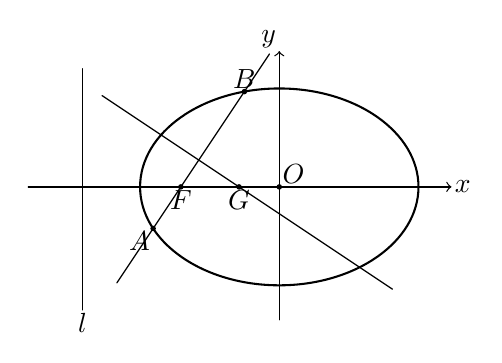
\begin{tikzpicture}[x=1.25cm,y=1.25cm,line cap=round,line join=round]
  \pgfmathsetmacro{\xA}{(-9-sqrt(26))/11}
  \pgfmathsetmacro{\yA}{3*(2-sqrt(26))/22}
  \pgfmathsetmacro{\xB}{(-9+sqrt(26))/11}
  \pgfmathsetmacro{\yB}{3*(2+sqrt(26))/22}
  \coordinate (A) at (\xA,\yA);
  \coordinate (B) at (\xB,\yB);
  \coordinate (F) at (-1,0);
  \coordinate (O) at (0,0);
  \coordinate (G) at (-9/22,0);
  \coordinate (M) at (-9/11,3/11); % midpoint of AB

  % Axes and left directrix l: x=-2.
  \draw[->,line width=0.45pt] (-2.55,0) -- (1.75,0);
  \draw[->,line width=0.45pt] (0,-1.35) -- (0,1.38);
  \draw[line width=0.45pt] (-2,-1.25) -- (-2,1.2);

  % Ellipse x^2/2+y^2=1.
  \draw[line width=0.75pt] (O) ellipse [x radius=1.4142,y radius=1];

  % One schematic secant through F and its perpendicular bisector.
  % The chosen slope only locates the drawing; it is not given data.
  \draw[line width=0.45pt] (-1.65,-0.975) -- (-0.1,1.35);
  \draw[line width=0.45pt] (-1.8,0.9273) -- (1.15,-1.0394);

  \fill (A) circle (1pt);
  \fill (B) circle (1pt);
  \fill (F) circle (1pt);
  \fill (O) circle (1pt);
  \fill (G) circle (1pt);

  \node[below left,inner sep=1pt]  at (A) {$A$};
  \node[above,inner sep=1pt]       at (B) {$B$};
  \node[below,inner sep=1pt]       at (F) {$F$};
  \node[above right,inner sep=1pt] at (O) {$O$};
  \node[below,inner sep=1pt]       at (G) {$G$};
  \node[above left,inner sep=1pt]  at (0,1.38) {$y$};
  \node[right,inner sep=1pt]       at (1.75,0) {$x$};
  \node[below,inner sep=1pt]       at (-2,-1.25) {$l$};
\end{tikzpicture}
